\documentclass{standalone}
\usepackage{xcolor}
\usepackage{verbatim}
\usepackage[T1]{fontenc}
\usepackage{graphics}
\usepackage{hyperref}
\newcommand{\code}[1]{\texttt{#1}}
\newcommand{\R}{R}
\newcommand{\pkg}[1]{#1}
\newcommand{\CRANpkg}[1]{\pkg{#1}}%
\newcommand{\BIOpkg}[1]{\pkg{#1}}
\usepackage{amsmath,amssymb,array}
\usepackage{booktabs}
\usepackage{subfig}
\usepackage{booktabs}
\usepackage{amsmath}
\usepackage{amssymb}
\usepackage{utfsym}
\usepackage{tikz}
\usetikzlibrary{shapes,arrows}
\tikzstyle{process} = [rectangle,draw=black!70,fill=white!30,rounded corners]
\tikzstyle{arrow} = [color=black,thick]
\newcommand{\class}[1]{`\code{#1}'}
\newcommand{\fct}[1]{\code{#1()}}
\numberwithin{equation}{section}
\DeclareMathOperator*{\argmin}{arg\,min}
\DeclareMathOperator*{\argmax}{arg\,max}
\def\E{{\mathbf E}}
\def\P{{\mathbf P}}
\def\x{{\bf x}}
\def\D{{\mathcal D}}
\def\O{{\mathcal O}}
\def\R{{\mathbb R}}
\def\S{{\cal S}}
\def\L{{\cal L}}
\def\B{{\mathbb{B}}}
\def\A{{\small\mathcal{A}}}
\def\C{{\small\mathcal{C}}}
\def\I{\mbox{I}}
\def\red{\color{black}}
\def\ind{{\perp \hspace{-0.2cm} \perp}}

\begin{document}
\nopagecolor
	\centering
	%\includegraphics{}
	% \resizebox{8cm}{!}{%
		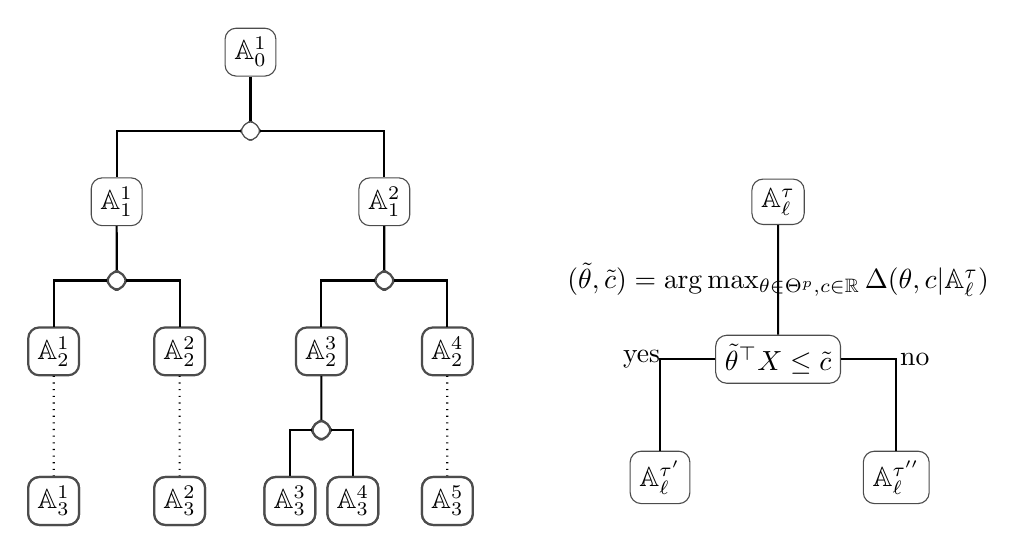
\begin{tikzpicture}[node distance=1cm,scale=0.6,
			edge from parent/.style={black,thick,draw},	
			edge from parent path={(\tikzparentnode) -| (\tikzchildnode)}]
			%ODT1
			\node (S01) [process] {$\mathbb{A}_0^1$};
			\node (N01) [process,below of=S01] {};
			\draw [arrow] (S01) -- (N01);
			\node (N01) [process,below of=S01] {}
			child {
				node (S11) [process,xshift=1cm] {$\mathbb{A}_1^1$};
				\node (N11) [process,below of=S11] {};
				\draw [arrow] (S11) -- (N11);
				\node (N11) [process,below of=S11] {}
				child {
					node (S21) [process, xshift=1cm ] {$\mathbb{A}_2^1$};
					\node (S31) [process, below of=S21,yshift=-0.9cm] {$\mathbb{A}_3^1$};
					%	\node (S31) [process, left of=S34,xshift=-2cm] {$\mathbb{A}_3^1$};
					\draw [dotted] (S21) -- (S31);%\hspace{4.5cm}
					\node (S31) [process, below of=S21,yshift=-0.9cm] {$\mathbb{A}_3^1$}
					%%
					%\node (N21) [process,below of=S21] {};
					%\draw [arrow] (S21) -- (N21);
					%\node (N21) [process,below of=S21] {}
					%child {
						%	node (S31) [process] {$\mathbb{A}_3^1$};
						%\draw [arrow] (S33) -- ++(0,-1.5);
						%	\node (S31) [process] {$\mathbb{A}_3^1$}
						%}
					%			child {
						%				node (S31) [process] {$\mathbb{A}_3^1$};
						%				\node (S31) [process] {$\mathbb{A}_3^1$}
						%			}
					%			child [missing] {}
					%			child {
						%				node (S32) [process] {$\mathbb{A}_3^2$};
						%				\node (S32) [process] {$\mathbb{A}_3^2$}
						%			}
				}
				child [missing] {}	
				child [missing] {}
				child [missing] {}
				child {
					node (S22) [process,xshift=-1cm] {$\mathbb{A}_2^2$};
					\node (S33) [process, below of=S22,yshift=-0.9cm] {$\mathbb{A}_3^2$};
					\draw [dotted] (S22) -- (S33);%\hspace{4.5cm}
					\node (S33) [process, below of=S22,yshift=-0.9cm] {$\mathbb{A}_3^2$}
					%%
					%\node (N22) [process,below of=S22] {};
					%\draw [arrow] (S22) -- (N22);
					%\node (N22) [process,below of=S22] {}
					%child {
						%	node (S33) [process] {$\mathbb{A}_3^2$};
						%	%\draw [arrow] (S33) -- ++(0,-1.5);
						%	\node (S33) [process] {$\mathbb{A}_3^2$}
						%}
				}
			}		
			child [missing] {}	
			child [missing] {}
			child [missing] {}	
			child [missing] {}
			child [missing] {}
			child {
				node (S12) [process, xshift=-1cm] {$\mathbb{A}_1^2$};
				\node (N12) [process,below of=S12] {};
				\draw [arrow] (S12) -- (N12);
				\node (N12) [process,below of=S12] {}
				child {
					node (S23) [process, xshift=1cm] {$\mathbb{A}_2^3$};
					\node (N23) [process,below of=S23] {};
					\draw [arrow] (S23) -- (N23);
					\node (N23) [process,below of=S23] {}
					child {
						node (S34) [process, xshift=0.5cm] {$\mathbb{A}_3^3$};
						%\draw [arrow] (S34) -- ++(0,-1.5);
						\node (S34) [process, xshift=0.5cm] {$\mathbb{A}_3^3$}
					}
					child [missing] {}
					child {
						node (S35) [process, xshift=-0.5cm] {$\mathbb{A}_3^4$};
						%\draw [arrow] (S35) -- ++(0,-1.5);
						\node (S35) [process, xshift=-0.5cm] {$\mathbb{A}_3^4$}
					}
				}
				child [missing] {}	
				child [missing] {}
				child [missing] {}
				child {
					node (S24) [process, xshift=-1cm] {$\mathbb{A}_2^4$};
					\node (S36) [process, below of=S24,yshift=-0.9cm] {$\mathbb{A}_3^5$};
					\draw [dotted] (S24) -- (S36);%\hspace{4.5cm}
					\node (S36) [process, below of=S24,yshift=-0.9cm] {$\mathbb{A}_3^5$}
					%%
					%\node (N24) [process,below of=S24] {};
					%\draw [arrow] (S24) -- (N24);
					%\node (N24) [process,below of=S24] {}
					%child {
						%	node (S36) [process] {$\mathbb{A}_3^5$};
						%\draw [arrow] (S36) -- ++(0,-1.5);
						%	\node (S36) [process] {$\mathbb{A}_3^5$}
						%}
					%			child [missing] {}
					% 			child {
						% 				node (S37) [process] {$\mathbb{A}_3^7$};
						% 				%\draw [arrow] (S37) -- ++(0,-1.5);
						% 				\node (S37) [process] {$\mathbb{A}_3^7$}
						% 			}
				}
			};
			%ODT2
			\node (input1) [process,right of=S12,xshift=4cm]{$\mathbb{A}_\ell^\tau$};
			\node (decision1) [process,below of=input1,yshift=-1cm] {$ \tilde \theta^\top X  \leq \tilde c$};
			\node (out1) [process,left of=decision1,xshift=-0.5cm,yshift=-1.5cm] {$\mathbb{A}_\ell^{\tau'}$};
			\node (out2) [process,right of =decision1,xshift=0.5cm,yshift=-1.5cm]{$\mathbb{A}_\ell^{\tau''}$};
			\draw [arrow] (input1) -- node {\bf $(\tilde \theta, \tilde c)=\mathop{\arg\max_{\theta\in\Theta^p, c\in\mathbb{R}}} {\Delta(\theta,c| \mathbb{A}_\ell^\tau)}$} (decision1);%\hspace{4.5cm}
			%\draw [arrow] (decision1) -| node[above=0.1mm]{yes} (out1);
			%\draw [arrow] (decision1) -| node[above=0.01mm]{no} (out2);
			\draw [arrow] (decision1) -| node {\color{black} yes  \ \ \ \ } (out1);%\Large
			\draw [arrow] (decision1) -| node {\color{black}\ \ \ \ no} (out2);%\Large
		\end{tikzpicture}
\end{document}
